\documentclass[border=0.2cm]{standalone}
 
% More defined colors
\usepackage[dvipsnames]{xcolor}
 
% Required package
\usepackage{tikz}
\usetikzlibrary{positioning}
 
 
\begin{document}
\tikzset{dspfilter/.append style = {minimum height=\dspfilterheight}}

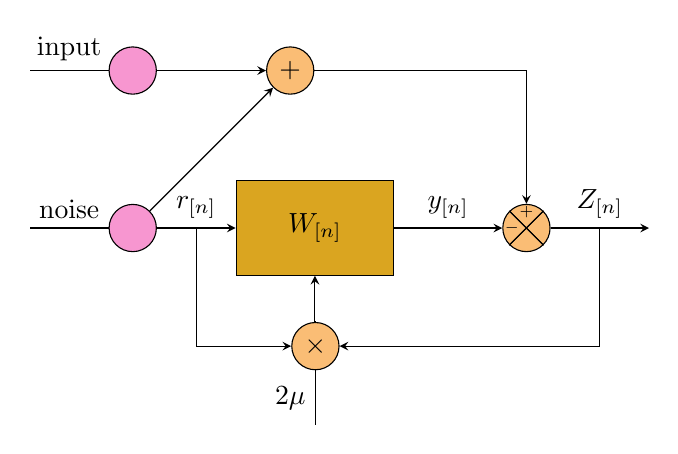
\begin{tikzpicture}

    % Sum shape
    \node[draw,
        circle,
        minimum size=0.6cm,
        fill=Rhodamine!50
    ] (inputt) at (0,2){};

    \node[draw,
        circle,
        minimum size=0.6cm,
        fill=Rhodamine!50
    ] (noise) at (0,0){};

    \node[draw,
        circle,
        minimum size=0.6cm,
        fill=BurntOrange!50
    ] (sum) at (2,2){};

    \node[draw,
        circle,
        minimum size=0.6cm,
        fill=BurntOrange!50
    ] (sum2) at (5,0){};

    \node[draw,
        circle,
        minimum size=0.6cm,
        fill=BurntOrange!50
    ] (mul) at (2.32,-1.5){};

    \draw (sum2.north east) -- (sum2.south west)
    (sum2.north west) -- (sum2.south east);

    \draw (sum2.north east) -- (sum2.south west)
    (sum2.north west) -- (sum2.south east);

    \node[above] at (sum2.center){\tiny $+$};
    \node[left=-1pt] at (sum2.center){\tiny $-$};
    \node at (sum.center){$+$};
    \node at (mul.center){$\times$};

    % Filter
    \node [draw,
        fill=Goldenrod,
        minimum width=2cm,
        minimum height=1.2cm,
        right=1cm of noise
    ]  (Filter) {$W_{[n]}$};

    % \node[left=of ns, fill=gray, circle, draw]
    % (mic) {};


    % Arrows with text label
    % \draw[-stealth] (noise.east) -- (Filter.west)
    % node[midway,above]{$e$};

    \draw[-stealth] (noise.east) -- (Filter.west)
    node[midway](noiise){}node[midway,above]{$r_{[n]}$};

    \draw[-stealth] (noiise.center) |- (mul.west);
    % \draw[-stealth] ()

    \draw[-stealth] (sum2.east) -- ++ (1.25,0)
    node[midway](output){}node[midway,above]{$Z_{[n]}$};

    \draw[-stealth] (output.center) |- (mul.east);

    \draw[-stealth] (sum.east) -| (sum2.north);

    \draw[-stealth] (noise.north east) -/ (sum.south west);

    \draw[-stealth] (inputt.east) -/ (sum.west);

    \draw[-stealth] (mul.north) -| (Filter.south);

    \draw[-stealth] (Filter.east) -- (sum2.west)
    node[midway,above]{$y_{[n]}$};

    % \draw (sum.west) -- ++(-1,0)
    % node[midway,above]{noise};

    \draw (inputt.west) -- ++(-1,0)
    node[midway,above]{input};

    \draw (noise.west) -- ++(-1,0)
    node[midway,above]{noise};

    \draw (mul.south) -- ++(0,-0.7)
    node[midway,left]{$2 \mu$};




\end{tikzpicture}

\end{document}